\documentclass[aima203_lecturenotes_ku.tex]{subfiles}

\setcounter{chapter}{5}
\begin{document}
\chapter{Numerical Differentiation and Numerical Integration}

In this chapter we shall be concerned with the problems of numerical differentiation and integration. We shall derive the formula to compute the following when only tabulated values of the function are known but the explicitly nature of the function is not known. Such scenario occurs in engineering in case of experimental data:

\begin{itemize}
\item $\displaystyle \frac{dy}{dx}, \; \frac{d^2y}{dx^2},\;...$ for any value of $x$ in $[x_0, x_n]$, and

\item $\displaystyle \int_{x_0}^{x_n} \; y\,dx$
\end{itemize}

\section{Numerical Differentiation}
The general method for deriving the numerical differentiation formulae is to differentiate the interpolating polynomial. Hence, corresponding to each of the Interpolating formula derived, we may derive a formula for the derivative.

\subsection{Newton's forward difference formulae}
The Newton's forward difference formula is:
\begin{equation}
  \label{newtforward6}
 \begin{gathered}
  y_n(x) = y_0 + u \Delta y_0 + \frac{u(u-1)}{2!}\, \Delta ^2 y_0 + \frac{u(u-1)(u-2)}{3!}\, \Delta ^3 y_0 + ... \\[1mm]
  + \frac{u(u-1)(u-2)...(u-(n-1))}{n!}\, \Delta ^n y_0
\end{gathered}
\end{equation}
where, $x=x_0 + uh$ and $h = x_{i+1} - x_{i}$. Differentiating ~\ref{newtforward6} with respect to $x$,

\begin{equation}
  \label{newtforwarddif}
  \begin{aligned}
    \frac{dy}{dx} =\frac{dy}{du} \frac{du}{dx} = \frac{1}{h} \left [ \Delta y_0 + \frac{2u -1}{2}\, \Delta^2\,  y_0 + \frac{3u^2-6u + 2}{6}\, \Delta^3 \, y_0 + ... \right ]
  \end{aligned}
\end{equation}
Differentiating ~\ref{newtforwarddif} with respect to $x$, we get,
\begin{equation}
  \label{newtforwarddif2}
  \begin{aligned}
    \frac{d^2y}{dx^2} = \frac{1}{h^2} \left [ \Delta^2 y_0 + \frac{6u -6}{6}\, \Delta^3 \,  y_0 + \frac{12u^2-36u + 22}{24}\, \Delta^4 \, y_0 + ... \right ]
  \end{aligned}
\end{equation}
These formulae are used for \textit{non-tabular} values of $x$. For tabular values of $x$, the formulae take simpler form. For $x=x_0$, we have $u=0$, and using this we can find the relations of $\displaystyle \left [ \frac{dy}{dx} \right ]  _{x=x_0} and \left [\frac{d^2y}{dx^2} \right ] _{x=x_0}$ which is in a simpler form.

\newpage
\subsection{Newton's backward difference formula}
In a similar way, different formulae can be derived by starting with other interpolation formulae. Thus, Newton's backward difference formula gives
\begin{equation}
  \label{newtbackwarddif}
  \left [ \frac{dy}{dx} \right ] _{x=x_n} = \frac{1}{h} \left [\nabla \, y_n + \frac{1}{2} \nabla ^2 \, y_n + \frac{1}{3} \nabla ^3 \, y_n + ... \right ]
\end{equation}
and

\begin{equation}
  \label{newtbackwarddif2}
  \left [ \frac{d^2y}{dx^2} \right ] _{x=x_n} = \frac{1}{h^2} \left [\nabla^2 \, y_n + \nabla ^3 \, y_n + \frac{11}{12} \nabla ^4 \, y_n + \frac{5}{6} \nabla ^5 \, y_n + ... \right ]
\end{equation}
\begin{remark}
   If the $x$-values of the data points are equally spaced then it is common to use Newton's interpolation.
\end{remark}
\subsection{Exercise}
Find the $dy/dx$ and $d^2y/dx^2$ at $x=1.2, \; x=1.6, \; x=2.2$ from the data: \\[1mm]
$(1, 2.7183), \; (1.2, 3.3201), \; (1.4, 4.0522), \; (1.6, 4.9530), \; (1.8, 6.0496), \; (2.0, 7.3891), \; (2.2, 9.0250)$.
\section{Numerical Integration}
The general problem of numerical integration may be stated as: Given a set of data points of a function $y=f(x)$, where $f(x)$ is not known explicitly, it is required compute the value of the definite integral $$I = \int_a^b \; y\,dx$$ As with the case of numerical differentiation, one replaces $f(x)$ by an interpolating polynomial $\phi(x)$ and obtains, on integration, an approximate value of the definite integral. Thus, different integration formulae can be obtained depending upon the type of the interpolation formula used. Approximating $y$ by Newton's forward difference formula, we obtained
$$ I = \int_{x_0}^{x_n} \; \left [ y_0 + p \Delta y_0 + \frac{p(p-1)}{2}\, \Delta^2 y_0 + \frac{p(p-1)(p-2)}{6}\, \Delta ^3 y_0 + ... \right ] \, dx$$
Since $x=x_0 +ph$, $dx = hdp$. When $x=x_0$, $p=0$ and $x=x_n$, $p=n$. Then,
$$ I = \int_{0}^{n} \; \left [ y_0 + p \Delta y_0 + \frac{p(p-1)}{2}\, \Delta^2 y_0 + \frac{p(p-1)(p-2)}{6}\, \Delta ^3 y_0 + ... \right ] \, h\,dp$$
Integrating we get,
\begin{equation}
  \label{numint}
  \begin{aligned}[b]
    I &= h \left [ py_0 + \frac{p^2}{2}\, \Delta y_0 + \left ( \frac{p^3}{3} - \frac{p^2}{2} \right ) \, \frac{\Delta^2 y_0}{2} +  \left ( \frac{p^4}{4} - p^3 + p^2 \right ) \frac{\Delta ^3 \, y_0}{6} + ... \right ]_0^n \\[1mm]
    &= nh \left [ y_0 + \frac{n}{2}\, \Delta y_0 + \left ( \frac{2n^2-3n}{12} \right ) \, \Delta^2\, y_0 +  \left ( \frac{n^3 - 4n^2 +4n}{24} \right ) \, \Delta ^3 \, y_0 + ... \right ]
  \end{aligned}
\end{equation}

This relation ~\ref{numint} is considered to be a general formula in the variable $n$. For a particular value of $n$ we get a particular formula. For example for $n=1$ we get the famous Trapezoidal rule and for $n=2$ and $n=3$ we get Simpson's 1/3 rule and Simpson's 3/8 rule respectively.

\subsection{Trapezoidal Rule}
Setting $n=1$ in the general formula ~\ref{numint}, all differences higher than the first will become zero and we obtained \\[1mm]
$\displaystyle \int_{x_0}^{x_1} \; y\,dx = h \left [ y_0 + \frac{1}{2} \Delta y_0 \right ] = h \left [ y_0 + \frac{1}{2}(y_1 -y_0) \right ] = \frac{h}{2}\, (y_0 + y_1).$ Similarly we can obtain \\[5mm] $\int_{x_1}^{x_2} \; y\,dx, ..... \int_{x_{n-1}}^n \; y\,dx $. Then we have,
\begin{equation}
  \label{trap}
  \begin{aligned}[b]
    \int_{x_0}^{x_n}\; y\,dx &= \int_{x_0}^{x_1} \; y\,dx + \int_{x_1}^{x_2} \; y\,dx + .... + \int_{x_{n-1}}^{x_n} \; y\,dx \\[1mm]
                             &= \frac{h}{2} \, (y_0 + y_1) + \frac{h}{2} \, (y_1 + y_2) + .... + \frac{h}{2} \, (y_{n-1} + y_n) \\[1mm]
                             &= \frac{h}{2} \, \{ y_0 + 2(y_1 + y_2 + ... + y_{n-1}) + y_n \}
  \end{aligned}
\end{equation}

\subsection{Simpson's 1/3-Rule}
Setting $n=2$ in the general formula ~\ref{numint}, all differences higher than the second will become zero and we obtained \\[1mm]
$\displaystyle \int_{x_0}^{x_2} \; y\,dx = 2h \left [ y_0 + \Delta \, y_0 + \frac{1}{6} \Delta^2 \, y_0 \right ] = \frac{h}{3}\, (y_0 + 4y_1 + y_2).$ Similarly we can obtain \\[5mm] $\int_{x_2}^{x_4} \; y\,dx, ..... \int_{x_{n-2}}^n \; y\,dx $. Then we have,
\begin{equation}
  \label{simp1}
  \begin{aligned}[b]
    \int_{x_0}^{x_n}\; y\,dx &= \int_{x_0}^{x_2} \; y\,dx + \int_{x_2}^{x_4} \; y\,dx + .... + \int_{x_{n-2}}^{x_n} \; y\,dx \\[1mm]
                             &= \frac{h}{3} \, (y_0 +4y_1 + y_2) + \frac{h}{3} \, (y_2 + 4y_3 + y_4) + .... + \frac{h}{3} \, (y_{n-2} + 4y_{n-1} + y_n) \\[1mm]
                             &= \frac{h}{3} \, \{ y_0 + 4(y_1 + y_3 + ... + y_{n-1}) + 2 (y_2 + y_4  ... + y_{n-2} ) + y_n \}
  \end{aligned}
\end{equation}

\begin{remark}
  It should be noted that this rule requires the division of the whole range into an even number of sub-intervals of width $h$.
\end{remark}

\subsection{Simpson's 3/8-Rule}
Setting $n=3$ in the general formula ~\ref{numint}, all differences higher than the third will become zero and we obtained \\[1mm]
$\displaystyle \int_{x_0}^{x_3} \; y\,dx = 3h \left [ y_0 + \frac{3}{2} \Delta \, y_0 + \frac{3}{4} \Delta^2 \, y_0 + \frac{1}{8} \Delta ^3 \, y_0 \right ] = \frac{3h}{8}\, (y_0 + 3y_1 + 3y_2+y_3).$ \\ Similarly we can obtain \\[5mm] $\int_{x_3}^{x_6} \; y\,dx, ..... \int_{x_{n-3}}^n \; y\,dx $. Then we have,
\begin{equation}
  \label{simp2}
  \begin{aligned}[b]
    \int_{x_0}^{x_n}\; y\,dx &= \int_{x_0}^{x_3} \; y\,dx + \int_{x_3}^{x_6} \; y\,dx + .... + \int_{x_{n-3}}^{x_n} \; y\,dx \\[1mm]
                             &= \frac{3h}{8} \, (y_0 +3y_1 + 3y_2 + y_3) + \frac{3h}{8} \, (y_3 + 3y_4 + 3y_5 + y_6) + .... + \frac{3h}{8} \, (y_{n-3} + 3y_{n-2} + 3y_{n-1} + y_n) \\[1mm]
                             &= \frac{3h}{8} \, \{ y_0 + 3(y_1 + y_2 + y_4 + y_5 + ... + y_{n-1}) + 2 (y_3 + y_6  ... + y_{n-3} ) + y_n \}
  \end{aligned}
\end{equation}

\subsection{Exercise}
\begin{enumerate}
\item Find, from the data, the area bounded by the curve and the $x$-axis: \\[1mm]
  $(7.47, 1.93), \; (7.48, 1.95),\; (7.49, 1.98),\; (7.50, 2.01),\; (7.51, 2.03),\; (7.52, 2.06)$

\item Find the volume of solid of revolution formed by rotating about the $x$-axis the area between the $x$-axis, the line $x=0$ and $x=1$, and a curve through the points: \\[1mm]
  $(0,1),\; (0.25,0.9896),\; (0.5,0.9589),\; (0.75,0.9089),\; (1,0.8415)$.4

\item Integrate $\displaystyle I = \int_0^{1.5}\; \frac{e^x +x}{sinx +1}\, dx$.

\item Evaluate: $\displaystyle I = \int_0^1 \; \frac{1}{1+x}\, dx$ using $h=0.125$.
\end{enumerate}

\section{Double Integration}
Formulae for the evaluation of double integral can be obtained by repeatedly applying the trapezoidal and Simpson's rules derived earlier.
\subsection{Trapezoidal Rule}
\begin{equation*}
  I = \int_{y_j}^{y_{j+1}}\; \int_{x_i}^{x_{i+1}} \; f(x,y)\;dx\,dy
\end{equation*}
where, $x_{i+1} = x_i + h$ and $y_{j+1} = y_j + k$.
By repeated application of trapezoidal rule to we get,
\begin{equation}
  \label{trapdouble}
  \begin{aligned}
    I &= \frac{h}{2} \,\int_{y_j}^{y_{j+1}}\; [f(x_i,y) + f(x_{i+1},y) ]\;dx\,dy \\[1mm]
      &= \frac{hk}{4} \, [f(x_i,y_j) + f(x_{i+1},y_j) + f(x_i,y_{j+1}) + f(x_{i+1},y_{j+1}) ]\;dx\,dy \\[1mm]
      &= \frac{hk}{4} \, [f_{i,j} + f_{i+1, j} + f_{i,j+1} + f_{i+1,j+1} ]\;dx\,dy
  \end{aligned}
\end{equation}

\subsection{Simpson's Rule}
\begin{equation*}
  I = \int_{y_{j-1}}^{y_{j+1}}\; \int_{x_{i-1}}^{x_{i+1}} \; f(x,y)\;dx\,dy
\end{equation*}
where, $x_{i+1} = x_i + h$ and $y_{j+1} = y_j + k$.
By repeated application of Simpson's rule to we get,
\begin{equation}
  \label{simpdouble}
  \begin{aligned}
    I &= \frac{h}{3} \,\int_{y_{j-1}}^{y_{j+1}}\; [f(x_{i-1},y) + 4f(x_i,y) + f(x_{i+1},y) ]\;dx\,dy \\[1mm]
      &= \frac{hk}{9} \, [f(x_{i-1},y_{j-1}) + 4f(x_{i-1},y_j) + f(x_{i-1},y_{j+1}) \\[1mm]
    & 4\{f(x_i,y_{j-1}) + 4f(x_i,y_j) + f(x_i,y_{j+1})\} + f(x_{i+1},y_{j-1}) + 4f(x_{i+1},y_j) + f(x_{i+1},y_{j+1})]
  \end{aligned}
\end{equation}
\vspace{1cm}

\begin{figure}[h]
  \centering
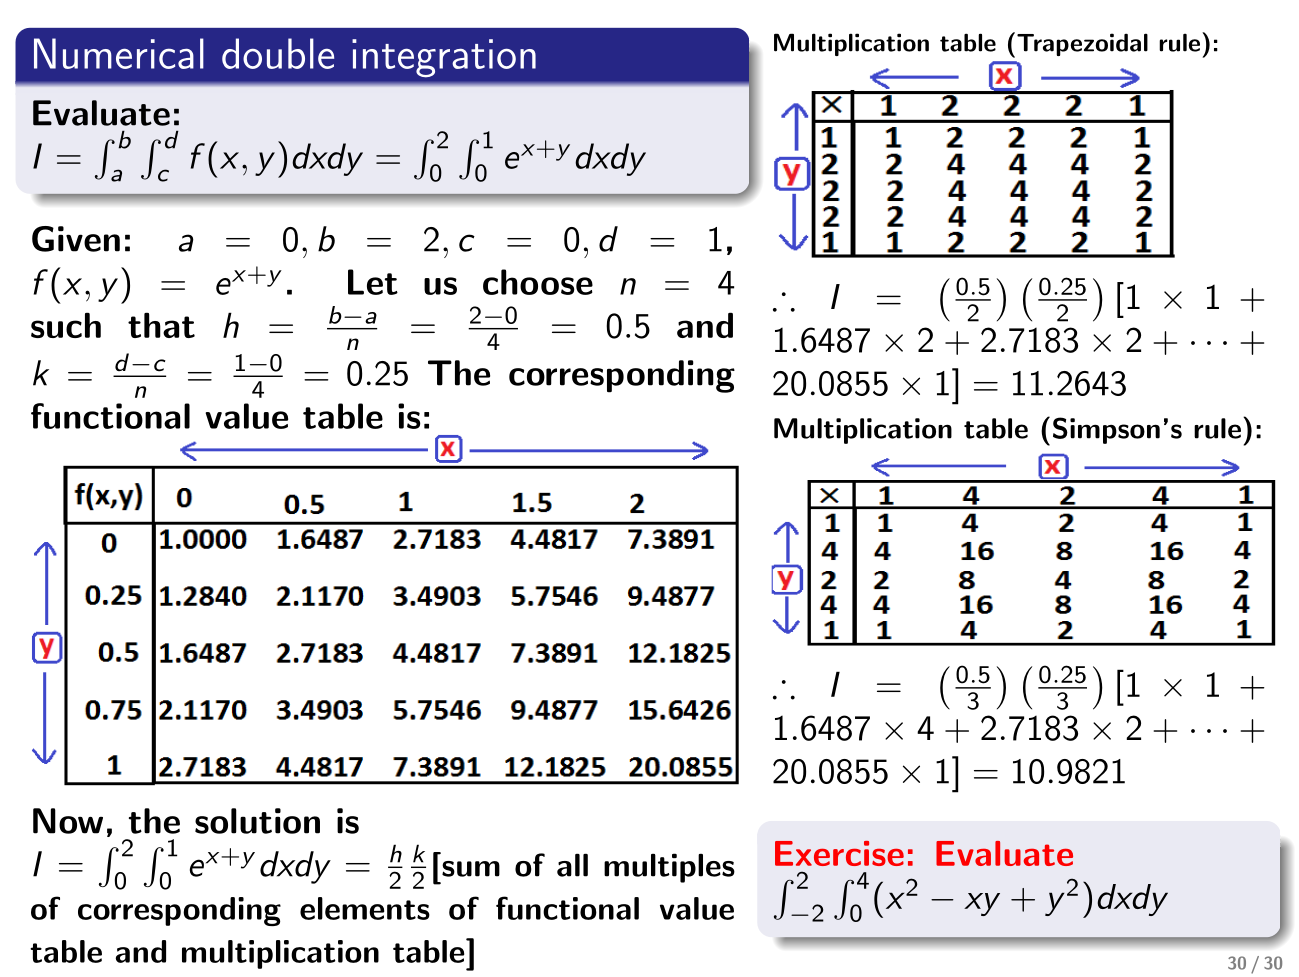
\includegraphics[width=15cm, height=11cm]{doubleint.png}
\end{figure}

\section{Romberg Integration}
This method can often be used to improve the approximate results obtained by the finite-difference methods. Its application to the numerical evaluation of definite integrals, for example in the use of trapezoidal rule, can be described, as follows.
\end{document}

%%% Local Variables:
%%% mode: LaTeX
%%% TeX-master: t
%%% End:
